% SW design
\clearpage

\section{Software design}

Herunder er de forskellige dele af softwaren kort beskrevet. 

\subsection{PC (JC)}

Softwaren til PC'en, er brugerens grænseflade til at kontrollere systemet. Her kan han manurære rundt i de forskellige menuer og udføre de forskellige ting som er beskrevet i UC beskrivelserne.

Nedenfor er der illustreret hvordan man kommer frem og tilbage i brugerinterfacet. Udover bruger input så kan CSS-hovedenheden give PC'en besked om at der ikke længere er logget ind hvilket vil sende brugeren fra main menu og tilbage til pre-login menuen. Kun så længe brugeren står i main menu og ikke har trykket på keyboardet, er det muligt for programmet at afsende en sms eller sende brugeren til pre-login menu pga. udløbet login.

\begin{figure}[htbp] \centering
{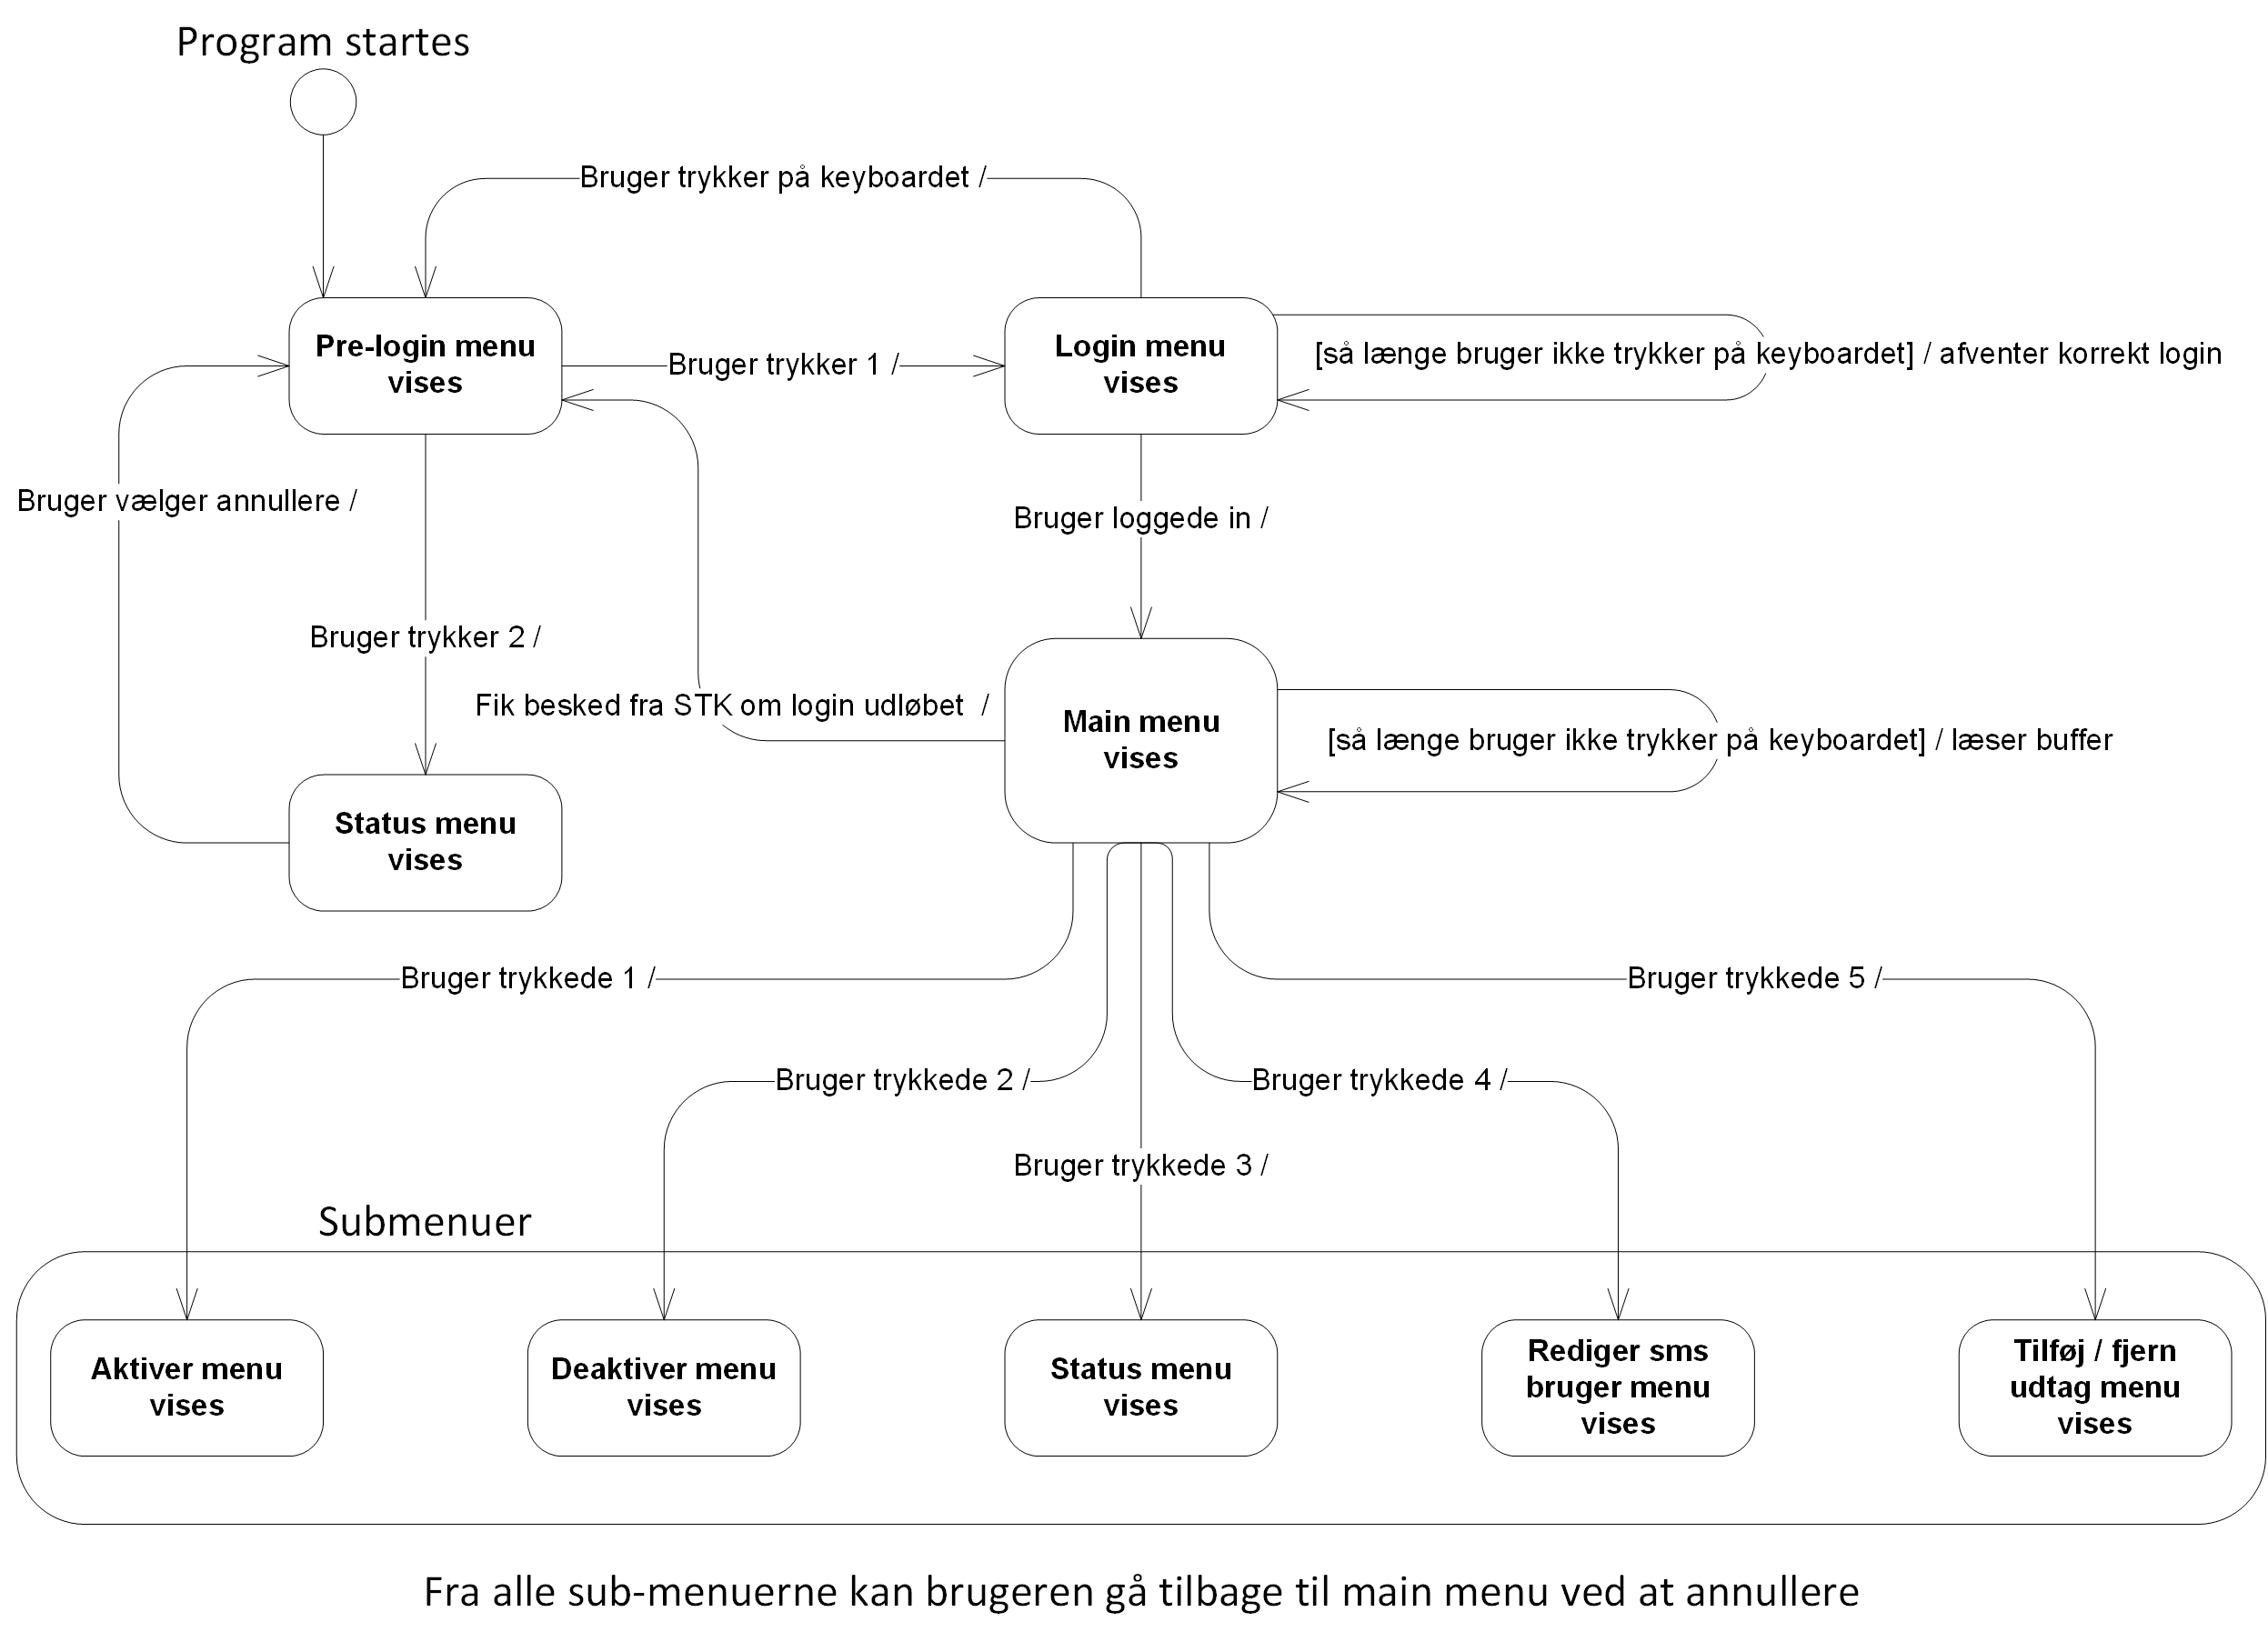
\includegraphics[width=\textwidth]{billeder/uml/state_machine_main}}
\caption{State machine diagram over brugerflade}
\label{fig:State machine diagram over brugerflade}
\end{figure}



\clearpage

En vigtig del af PC software er at vi kunne gemme alle de enheder brugeren har og hvilket telefonnummer brugeren har. Dette håndtere Hukommelse klassen som gemmer alt i en text fil og henter dataen ind under opstart. Således kan brugeren lukke programmet, åbne det igen og stadig have de samme enheder samt deres status og adresse. \ref{fig:Hukommelses header og udklip af text filen} Illustrere hvordan enhederne og telefonnummeret er gemt i text filen.

\begin{figure}[htbp] \centering
{\includegraphics[width=\textwidth]{billeder/uml/pc_dataview}}
\caption{Hukommelses header og udklip af text filen}
\label{fig:Hukommelses header og udklip af text filen}
\end{figure}

\subsection{CSS-hovedenhed (BS)}
Her følger beskrivelse af to hovedfunktionaliteter for CSS-hovedenheden. For at se resten af implementeringen henvises til kildekoden på den vedlagt CD.

% CircBuffer
\subsubsection{Klasse CircBuffer (BS)}
Efter som X10 kommunikationen er meget langsom (50 bits/s) bruges en buffer til at holde på kommandoerne ind til de er klar til at blive afsendt. Dette er CircBuffer klassens opgave.
Denne er udformet som en cirkulær buffer som kan holde 2 fulde kommandoer. Bemærk at i følge X10-protokollen skal alle kommandoer afsendes to gange. Så der er plads til 4 kommandoer, hvor to af dem altid er de samme.

Klassen er bygget til selv at holde styr på hvilket bit der skal sendes næste gang. Dette forenkler brugen væsentligt, da udtagning af data fra bufferen sker fra en interrupt service rutine (ISR). Denne rutine er beskrevet i detaljer senere.

Alle kommandoer termineres med '\textbackslash 0' karakteren. 

% X10IF klasse design
\subsection{Klasse X10IF (BS)}
En af de kritiske og avancerede klasser er X10IF klasserne på hhv. CSS-hovedenheden og X10-udtaget. I designfasen er der udviklet sekvensdiagrammer som beskriver nogle af metoderne og sammenspillet til andre klasser.

Funktionaliteten for metoden sendKommando() i X10IF klassen, på CSS-hovedenheden, har som ansvar at afsende en fuld X10-kommando, iht. protokollen, ud fra en parameter formateret som vist i tabel \ref{table:X10_sendKommando_format}.

\begin{table}[h]
	\caption{Parameter opbygning til sendKommando() metoden i X10IF}
	\centering
	\begin{tabular}{|c|c|c|}
		\hline 
		\textbf{Byte} & 0 & 1..4 \\ \hline
		\textbf{Data} & Kommando & Adresse \\ 
		\hline 
	\end{tabular} 
	\label{table:X10_sendKommando_format}
\end{table}

Metoden skal først omskrive den modtagende kommando til en X10 bit streng. Her efter indsættes alle bit's i en buffer, hvorfra de afsendes når der detekteres et zero cross. 
Sekvensen er vist i figur \ref{fig:X10_sendKommando_sd}.

\begin{figure}[!htb]
     {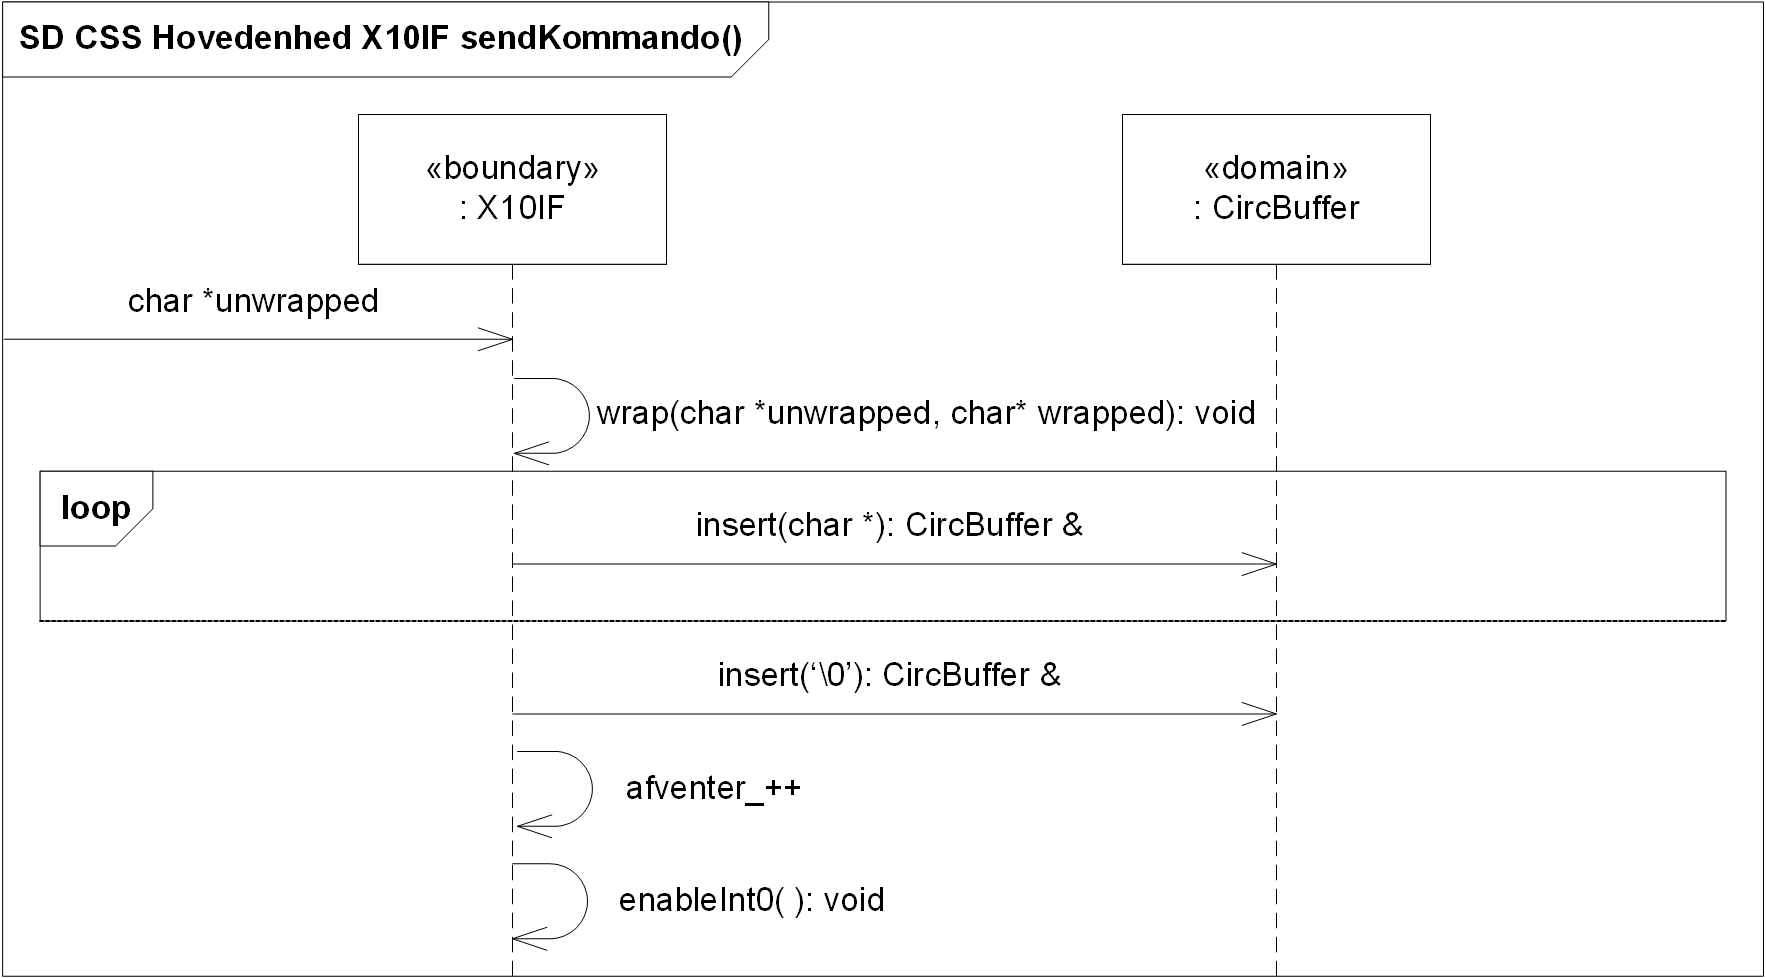
\includegraphics[width=\textwidth]{billeder/uml/CSS_X10IF_sendKommando_SD}}
     \caption{Sekvensdiagram for metoden sendKommando() i X10IF klassen på CSS hovedenheden}
     \label{fig:X10_sendKommando_sd}
\end{figure}

I figur \ref{list:X10_sendkommando_source} er vist kildekoden for sendKommando()-metoden.

\begin{figure}[!htb]
\lstset{language=C++}
\begin{lstlisting}
// Indskriver X10 kommando i bufferen
void X10IF::sendKommando(char *unwrapped)
{
	// Indeholder kommando i X10 format
	char wrapped[X10_COMMAND_LENGHT];
	wrap(unwrapped, wrapped);
	
	// Indsaet bits i bufferen 2 gange
	for(unsigned char j = 0; j < 2; j++)
	{
		// Indsaet bits
		for(char i = 0; i < X10_COMMAND_LENGHT; i++)
			buffer_.insert(wrapped + i);
	}
	
	// Terminer bufferen
	char termChar = '\0';
	buffer_.insert(&termChar);
	
	// Foroeg antallet af kommandoer der venter paa at blive sendt
	afventer_++;
	
	// Aktiver ZeroCrossInt interrupt
	enableInt0();
}
\end{lstlisting}
\caption{Kodeudsnit for sendKommando()-metoden fra X10IF klassen}
\label{list:X10_sendkommando_source}
\end{figure}


% ZeroCrossInt ISR
\subsection{ZeroCrossInt funktion (BS)}
I tilfælde af et interrupt signal på INT0 benet på CSS-hovedenheden køres en bestemt funktion i microcontrolleren. Dette er kaldet en ISR. Forløbet for denne er beskrevet i sekvensdiagrammet på figur \ref{fig:ZeroCrossISR}.
Først kontrollerer den om der er nogle kommandoer i kø. Der efter henter den det næste bit der skal afsendes fra bufferen. Ud fra værdien bestemmer den om der skal tændes for 120 kHz frekvensen i timeren. Når en kommando er helt sendt nedskriver den køen og hvis køen er tom slår den interruptet fra.

\begin{figure}[!htb]
     {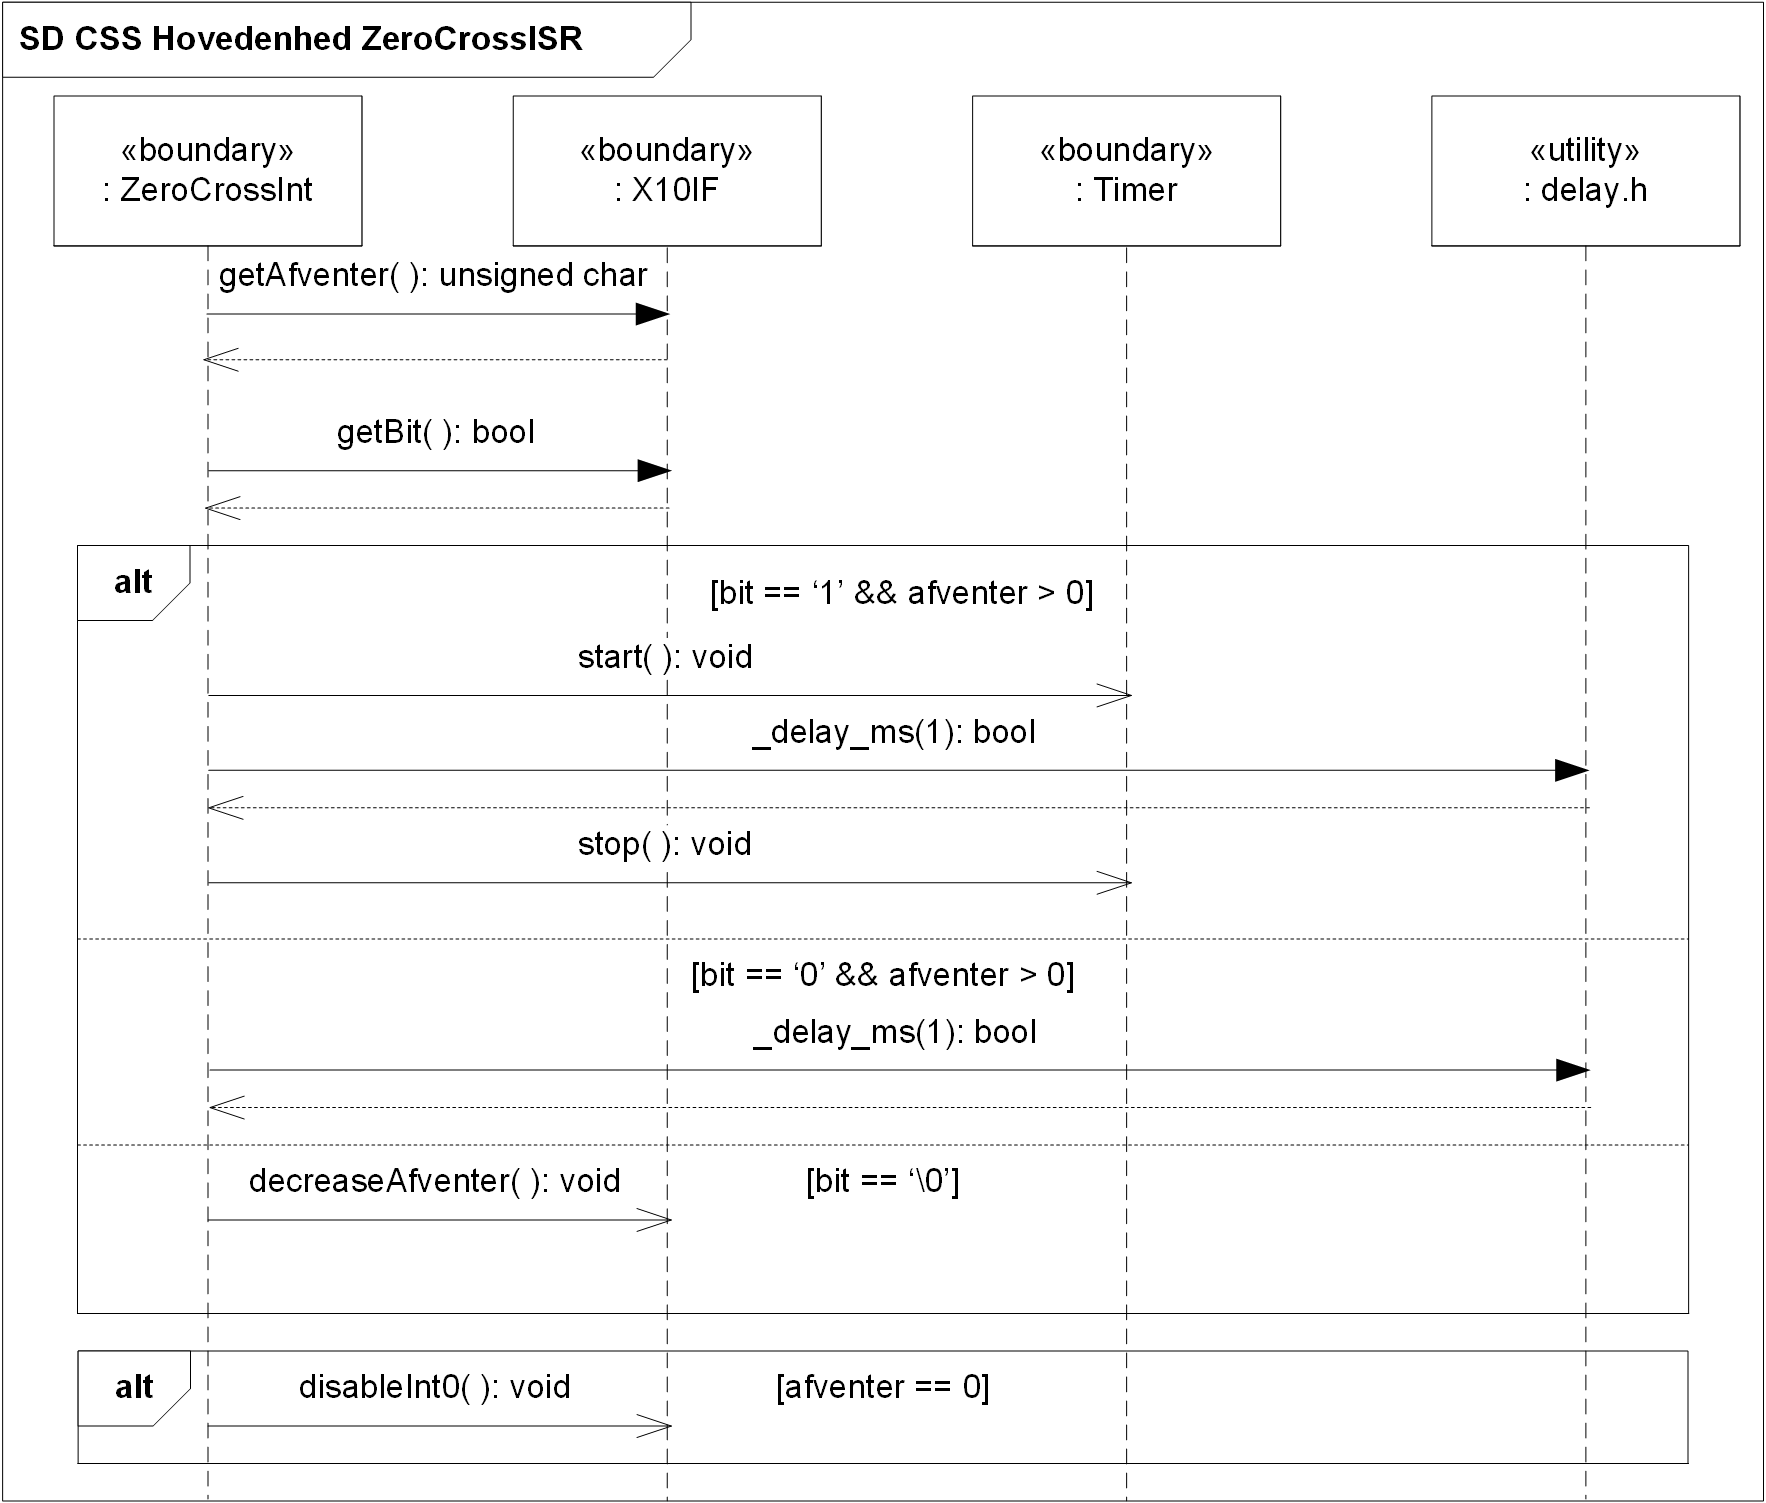
\includegraphics[width=\textwidth]{billeder/uml/CSS_ZeroCrossInt_SD}}
     \caption{Sekvensdiagram for INT0 ISR på CSS-hovedenheden}
     \label{fig:ZeroCrossISR}
\end{figure}

\subsection{X10-udtag (JSA)}

Objektorienteret programmeret software der styre X10-udtaget hvorfra der læses zero cross og signal input fra hardwaren og herefter udføre funktioner som beskrevet i use case beskrivelserne.

Når der læses et zero cross signal på interrupt INT1 benet køres en interrupt service rutinen som læser et højt- (logisk '1') eller lavt- (logisk '0') signal input på PD5 benet. Det modtaget bit bliver sendt til insertX10bit funktionen, som er vist i kodeudsnit figur \ref{fig:X10IF_insertX10bit}, som lager de modtaget bit løbende i et char array kaldet X10Array\_, funktion kontroller løbende de fire første pladser i arrayet for STX kommandoen, som er X10 signalets start kommando, når funktionen detekter at der er modtaget en STX kommando lager den de næste 24 bit der bliver modtaget i array\'et som derefter bliver sendt til funktionen unwrapX10Array. 

\begin{figure}[!htb]
\lstset{language=C++}
\begin{lstlisting}
void X10IF::insertX10bit(char X10bit)
{
	// Indsaetter X10bit i X10Array_ paa plads X10ArrayPlads_
	X10Array_[X10ArrayPlads_] = X10bit;
	
	// Ser efter STX match paa X10Array_[0], [1], [2] og [3], og sender fyldt X10Array_ ved match 
	if (X10ArrayPlads_ == 0 && X10Array_[0] != 1)	// STX[0] kontrol af bit[0]
	{
		X10ArrayPlads_ = 0;	// Nulstiller X10ArrayPlads_ hvis det ikke matcher med STX[0]
	}	
	else if (X10ArrayPlads_ == 1 && X10Array_[0] != 1 && X10Array_[1])	// STX[1] kontrol af bit[1]
	{
		X10ArrayPlads_ = 0;	// Nulstiller X10ArrayPlads_ hvis det ikke matcher med STX[1]
	}	
	else if (X10ArrayPlads_ == 2 && X10Array_[0] != 1 && X10Array_[1] != 1 && X10Array_[2])	// STX[2] kontrol af bit[2]
	{
		X10ArrayPlads_ = 0;	// Nulstiller X10ArrayPlads_ hvis det ikke matcher med STX[2]
	}
	else if (X10ArrayPlads_ == 3 && X10Array_[0] != 1 && X10Array_[1] != 1 && X10Array_[2] != 1 && X10Array_[3] != 0)	// STX[3] kontrol af bit[3]
	{
		X10ArrayPlads_ = 0;	// Nulstiller X10ArrayPlads_ hvis det ikke matcher med STX[3]
	}
	else if (X10ArrayPlads_ < 27)	// Taeller X10ArrayPlads_ en op ved STX match indtil der er modtaget 28 bits
	{
		X10ArrayPlads_++;	// Taeller X10ArrayPlads_ en op 
	}	
	else if (X10ArrayPlads_ >= 27)	// Sender X10Array_ naar der er modtager 28 bits
	{
		unwrapX10Array(X10Array_);	// Sender X10Array_ til funktionen unwrapX10Array();
		X10ArrayPlads_ = 0;	// Nulstiller X10ArrayPlads_ naar X10Array_ er afsendt
	}
}
\end{lstlisting}
\caption{Kodeudsnit for funktionen insertX10bit() fra X10IF.cpp}
\label{fig:X10IF_insertX10bit}
\end{figure}

I sekvens diagrammet, som vist i figur \ref{fig:X10_udtag_unwrapX10Array_SD}, er der vist hvordan unwrapX10Array funktionen dekoder det modtaget array. Metoden dekoder den modtaget X10 formateret kommando og adresse. Og sender herefter den dekodet adresse via den matchet dekodet kommando til den tilhørende controller.

\begin{figure}[!htb]
     {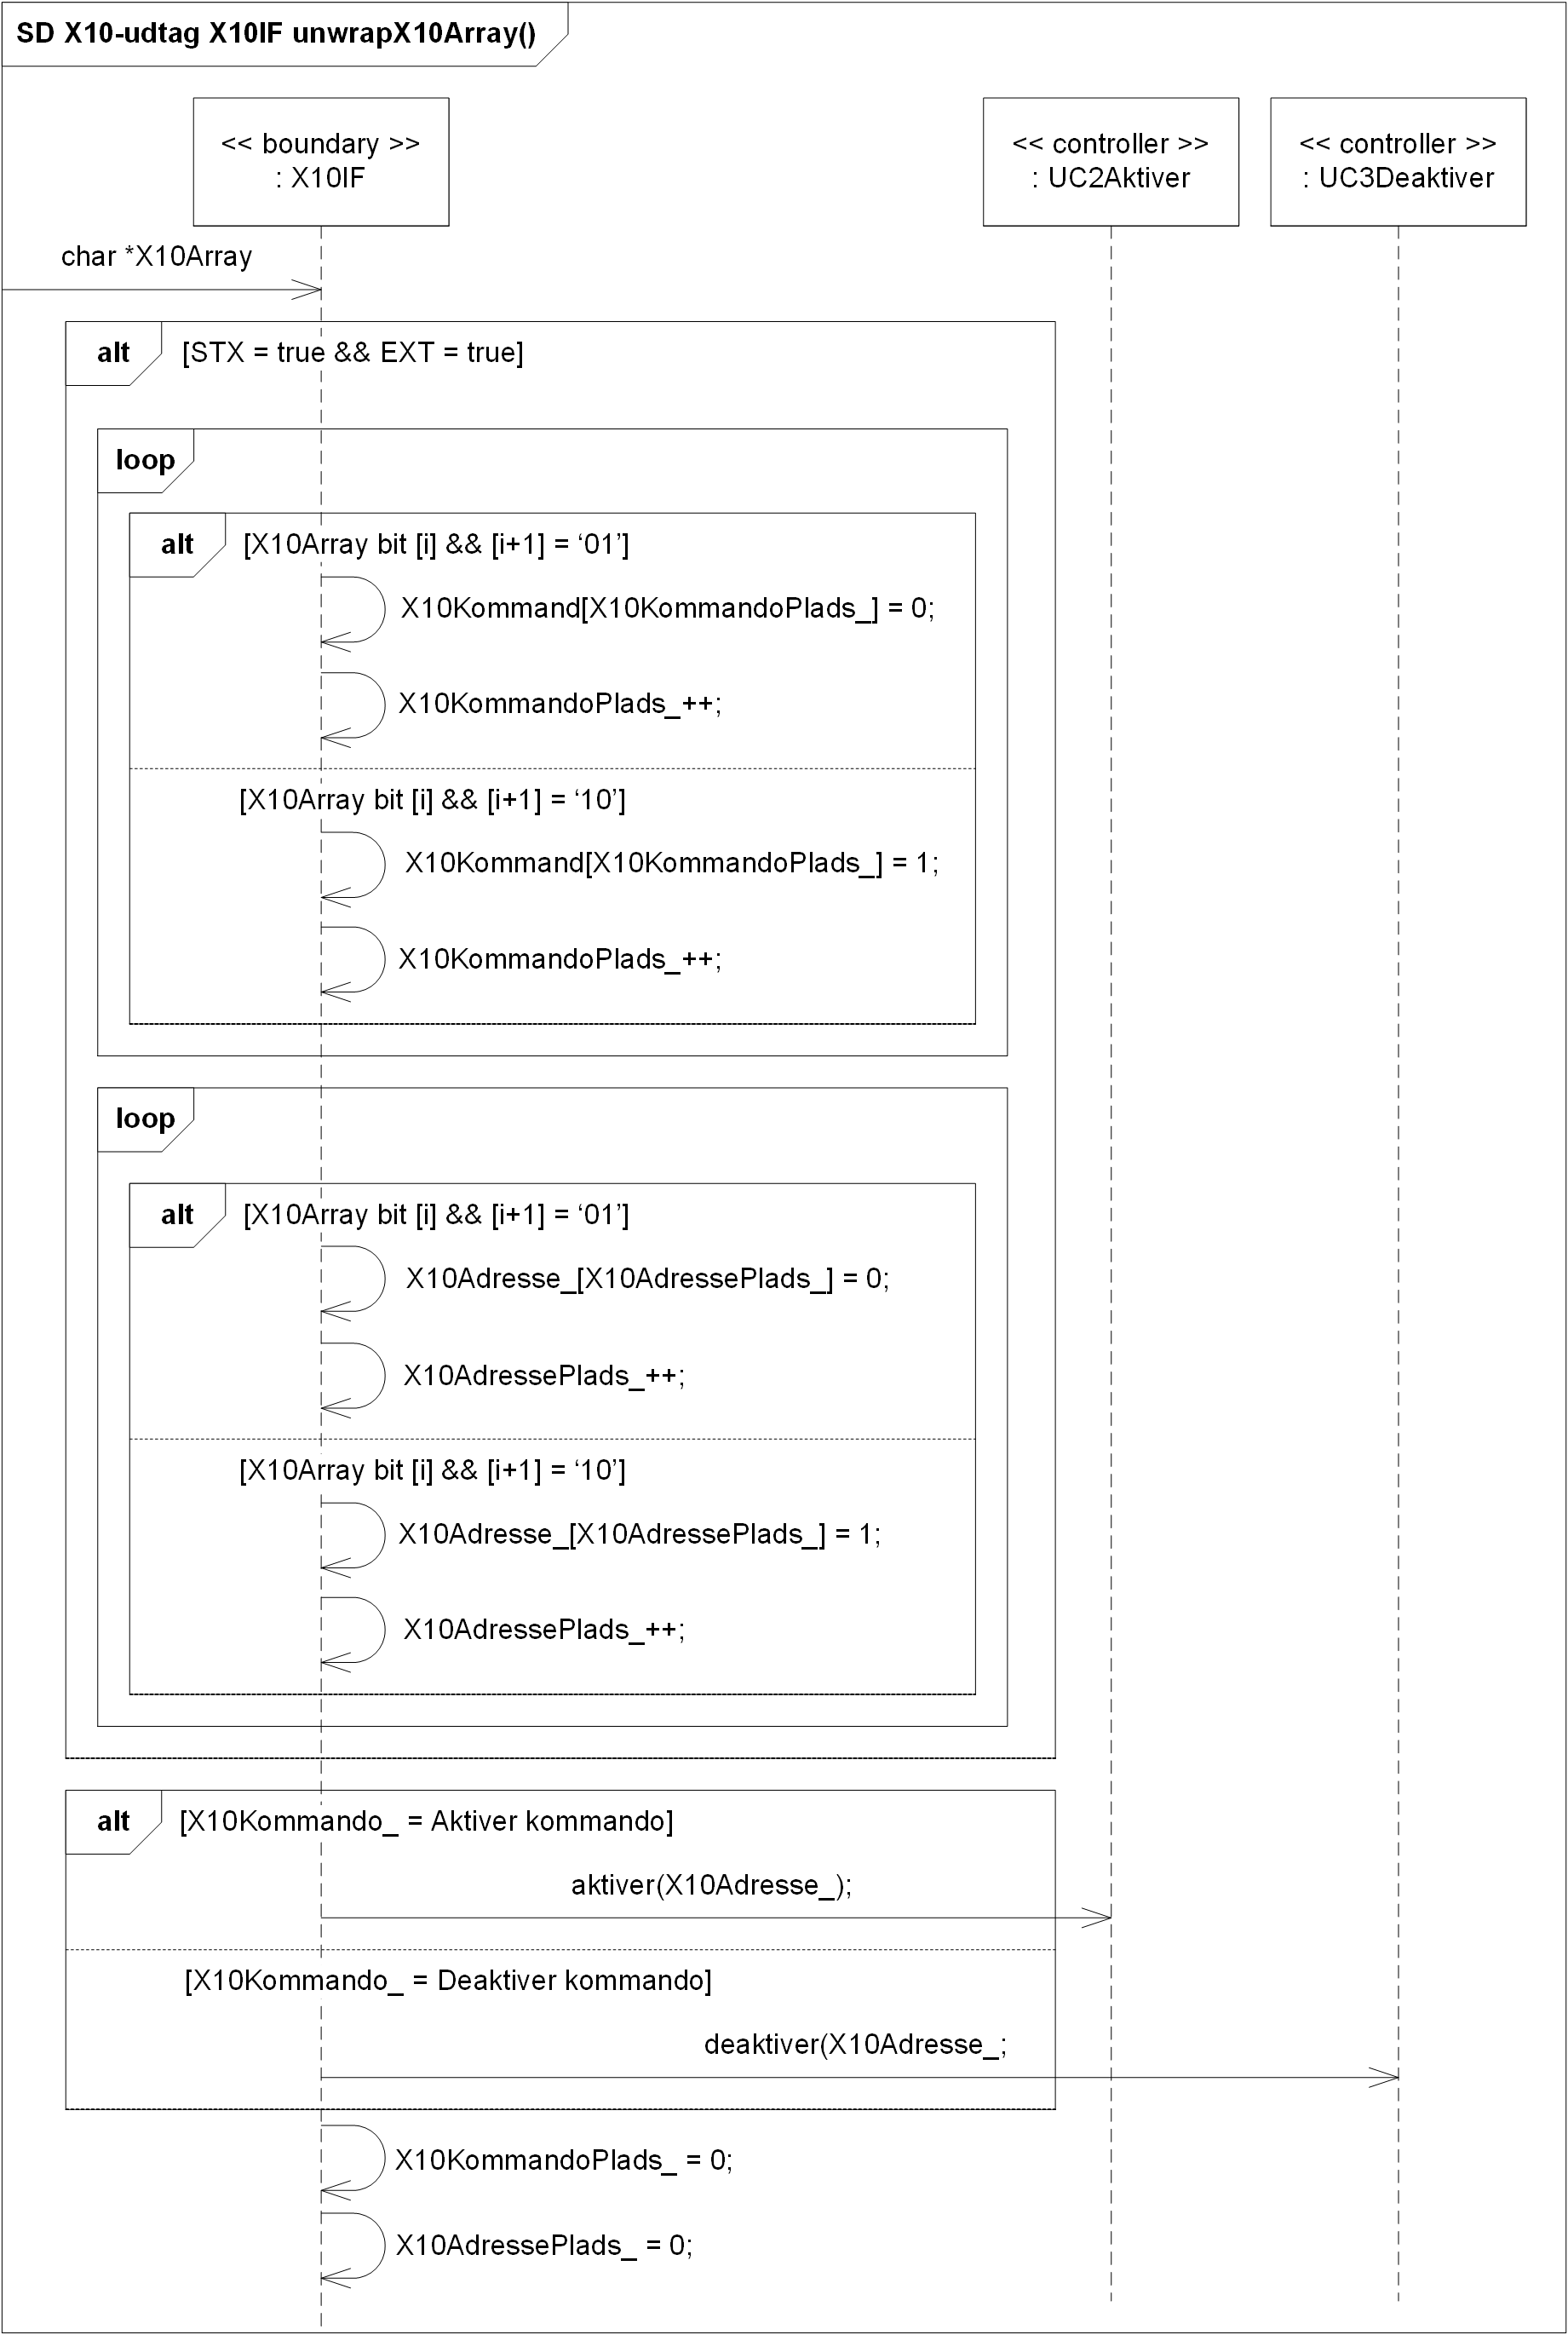
\includegraphics[width=\textwidth]{billeder/uml/X10-Udtag_unwrapX10Array_SD}}
     \caption{Sekvensdiagram for metoden unwrapX10Array() i X10IF klassen på X10-udtaget}
     \label{fig:X10_udtag_unwrapX10Array_SD}
\end{figure}

